\documentclass{article}
\usepackage{graphicx}
\setlength{\parindent}{0cm}

\usepackage{listings}
\usepackage{color}

\definecolor{dkgreen}{rgb}{0,0.6,0}
\definecolor{gray}{rgb}{0.5,0.5,0.5}
\definecolor{mauve}{rgb}{0.58,0,0.82}

\lstset{frame=tb,
  language=Matlab,
  aboveskip=3mm,
  belowskip=3mm,
  showstringspaces=false,
  columns=flexible,
  basicstyle={\small\ttfamily},
  numbers=none,
  numberstyle=\tiny\color{gray},
  keywordstyle=\color{blue},
  commentstyle=\color{dkgreen},
  stringstyle=\color{mauve},
  breaklines=true,
  breakatwhitespace=true
  tabsize=3
}

\begin{document}

\title{Python Fuzzy Clustering}
\author{Barney Tannahill and Kyle Kastner}

\maketitle

\section*{K-means and Fuzzy C-means, Continued}
Continuing the investigation from last homework, we applied the K-means and 
Fuzzy C-means algorithms to various datasets and visualized the resulting clusters.
Our outcomes were comparable to the results obtained from the MATLAB tests. 

\section*{Datasets}
\subsection*{Breast Cancer Data}
The data set used for this exercise consists of 569 different breast cancer diagnoses. 
Each diagnosis contains 30 additional measurement parameters. 

\subsubsection*{Hard K Means Clustering Results}
In an attempt to generate a classification method to identify benign and 
malignant diagnoses based solely on the gathered parameters, the Hard K Means
algorithm available from the scipy library. The number of clusters was selected
as 2 to account for the two possible diagnoses included in the data set.
Figure ~\ref{fig:f0} shows the distribution of samples between the two clusters
with the dimension of the data reduced to two in order to better display the data.
\begin{figure}[h!]
\caption{Distribution of samples}
  \centering
    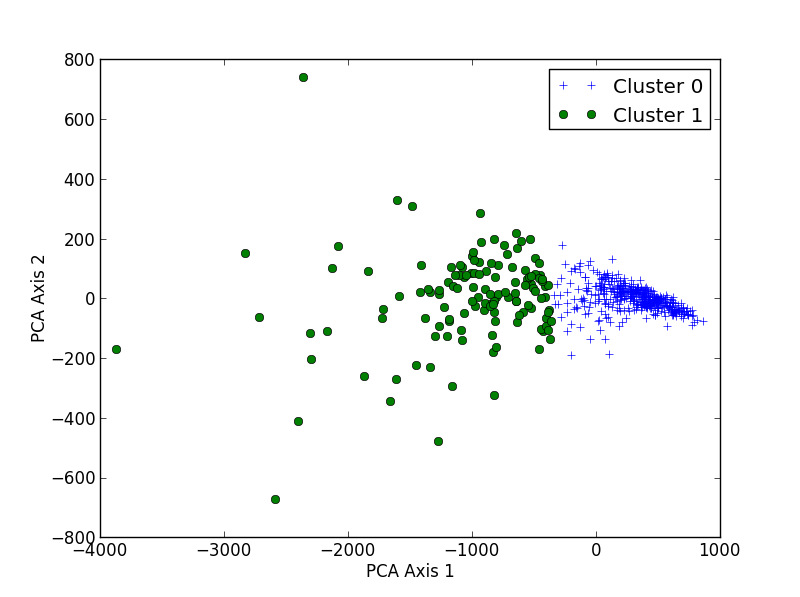
\includegraphics[width=0.85\textwidth]{figure_0.png}
  \label{fig:f0}
\end{figure}
These additional statistics were calculated to help show the effectiveness of 
the clustering method at classifying the diagnosis data as benign or malignant:
\vspace*{1\baselineskip}      
\begin{verbatim}
True Malignant Identification (%): 0.992
False Malignant Identification (%): 0.00763
True Benign Identification (%): 0.187
False Benign Identification (%): 0.813
\end{verbatim}
\vspace*{1\baselineskip}      
These statistics show that the categorization is accurate when it identifies 
a sample as part of the malignant cluster; however, it is not as accurate at identifying benign diagnoses.
\subsubsection*{Fuzzy C Means Clustering Results}
Next, the Fuzzy C Means algorithm was used to attempt to categorize the data 
into two clusters.  To gauge whether or not the resulting clusters could 
predict whether or not the cancer was benign or not, the following statistics were calculated:
\vspace*{1\baselineskip}      
\begin{verbatim}
Avg Value for Cluster 0 Given Diagnosis Benign (Result = 0): 0.975
Avg Value for Cluster 1 Given Diagnosis Benign (Result = 0): 0.025
Avg Value for Cluster 0 Given Diagnosis Malignant (Result = 1): 0.419
Avg Value for Cluster 1 Given Diagnosis Malignant (Result = 1): 0.581
\end{verbatim}
\vspace*{1\baselineskip}      
\begin{verbatim}
Standard Deviation Value for Cluster 0 Given Diagnosis Benign (Result = 0): 0.0480
Standard Deviation Value for Cluster 1 Given Diagnosis Benign (Result = 0): 0.0480
Standard Deviation Value for Cluster 0 Given Diagnosis Malignant (Result = 1): 0.377
Standard Deviation Value for Cluster 1 Given Diagnosis Malignant (Result = 1): 0.377
\end{verbatim}
\vspace*{1\baselineskip}      
This data shows a strong association between benign diagnoses and points 
close to Cluster 0.  The association between malignant diagnoses and Cluster 1 was present, but not as strong.
Although these statistics are interesting, what is of immediate interest is 
the chance of a diagnosis being malignant or benign based on the value of the 
cluster membership functions, not the other way around.  In order to calculate 
this, the average diagnosis based on different possible cluster membership 
function threshold values was used.  Figures ~\ref{fig:f1} and ~\ref{fig:f2} 
show the chance of positively (accurately) identifying a diagnosis as benign 
or malignant based on the cluster value (for Cluster 0 and 1, respectively).
\begin{figure}[h!]
  \centering
    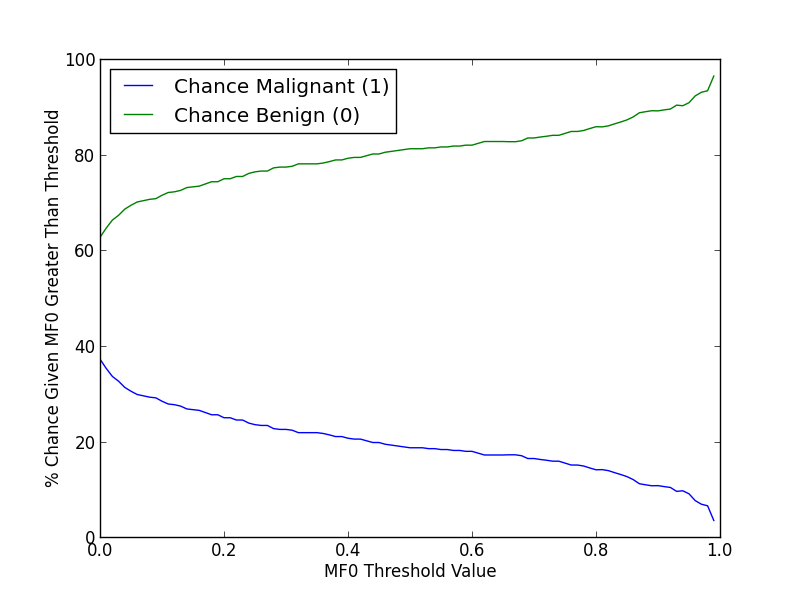
\includegraphics[width=0.85\textwidth]{figure_1.png}
  \label{fig:f1}
\end{figure}

\begin{figure}[h!]
  \centering
    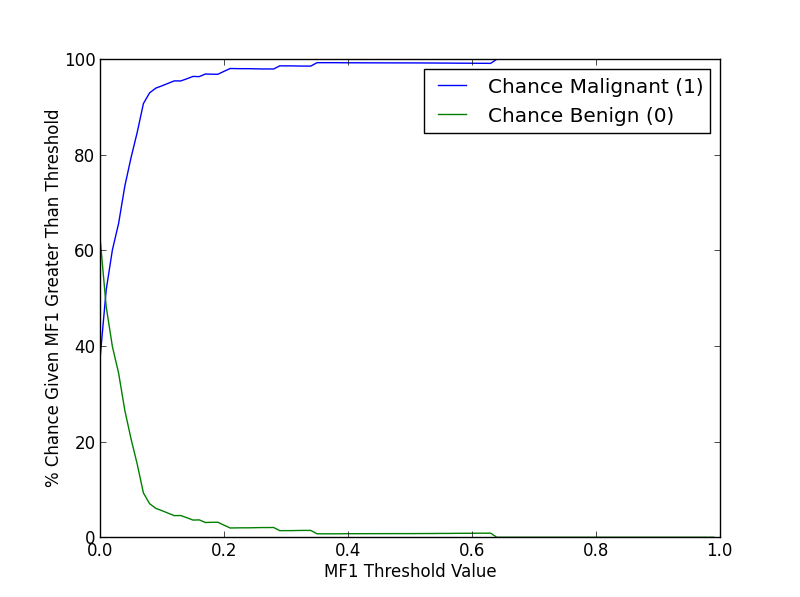
\includegraphics[width=0.85\textwidth]{figure_2.png}
  \label{fig:f2}
\end{figure}

\begin{figure}[h!]
  \centering
    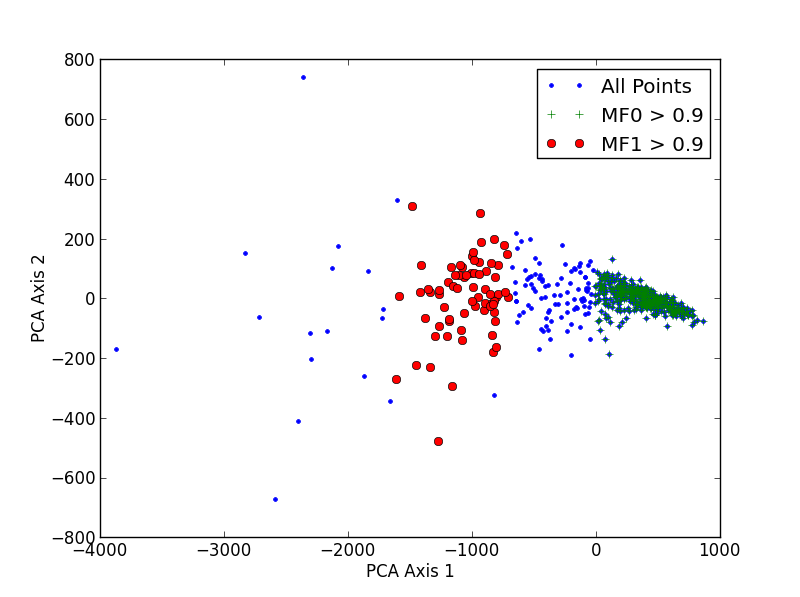
\includegraphics[width=0.85\textwidth]{figure_3.png}
  \label{fig:f3}
\end{figure}

\subsection*{MNIST Digits}
Testing was also performed on the MNIST digits dataset, as seen in 
Figure ~\ref{fig:f4}.
To perform this analysis, a size (1738,64) matrix of 8x8 images were PCA 
projected to (1738,2), then analyzed with both K-means and Fuzzy C Means algorithms.
Though this dataset did not cluster as well as the cancer set, there is clearly some regionality
to the results. One can imagine an 8 and 3 being very near to each other, while
0 and 1 are very likely to be far apart. This theme will continue in the next homework.
\begin{figure}[h!]
    \caption{Clustered digits}
  \centering
    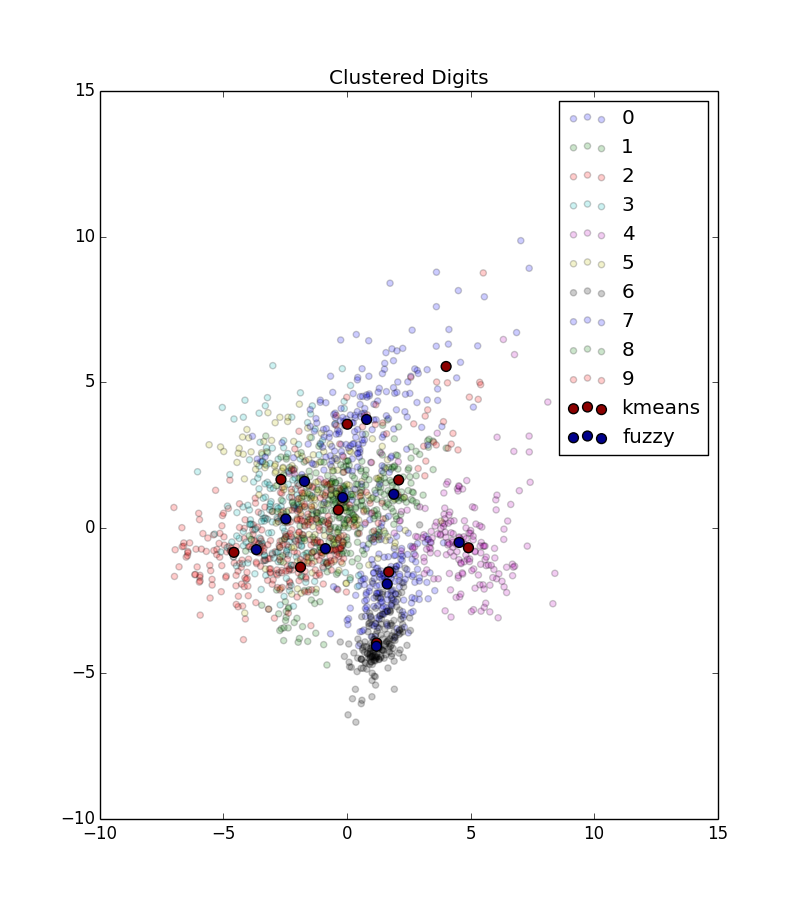
\includegraphics[width=0.85\textwidth]{digitscluster.png}
  \label{fig:f4}
\end{figure}

\begin{thebibliography}{9}
\bibitem{BCDiagnostic}
  Dr. William H. Wolberg, W. Nick Street, Olvi L. Mangasarian 
  \emph{Breast Cancer Wisconsin (Diagnostic) Data Set}
  UCI Machine Learning Repository 
  http://archive.ics.uci.edu/ml/datasets/Breast+Cancer+Wisconsin+i\%28Diagnostic\%29
                                                                                        
\bibitem{scipy}
  \emph{K-means clustering with scipy}
  The Glowing Python
  http://glowingpython.blogspot.com/2012/04/k-means-clustering-with-scipy.html
                                                                                        
\bibitem{skfuzzy}
  \emph{Sci-kit Fuzzy Library}
  https://github.com/scikit-fuzzy                       
                                                                                        
\bibitem{iris}
    \emph{Comparison of LDA and PCA 2D projection of Iris Dataset}
    http://scikit-learn.org/stable/auto\_examples/decomposition/plot\_pca\_vs\_lda.html\#example-decomposition-plot-pca-vs-lda-py

\bibitem{mnist}
    Y. LeCun, C. Cortes, C. Burges
    \emph{The MNIST database of handwritten digits}
    http://yann.lecun.com/exdb/mnist/

\end{thebibliography}
\end{document}
